\documentclass{beamer}
\usepackage{ctex, hyperref}
\usepackage[T1]{fontenc}

% other packages
\usepackage{latexsym,amsmath,xcolor,multicol,booktabs,calligra}
\usepackage{graphicx,pstricks,listings,stackengine}
\usepackage[normalem]{ulem}

\author{userElaina}
\title{一些探索}
\institute{School of AI}
\date{2024.06.09}
\usepackage{JilinUniv}

\def\cmd#1{\texttt{\color{red}\footnotesize $\backslash$#1}}
\def\env#1{\texttt{\color{blue}\footnotesize #1}}
\definecolor{deepblue}{rgb}{0,0,0.5}
\definecolor{deepred}{rgb}{0.6,0,0}
\definecolor{deepgreen}{rgb}{0,0.5,0}
\definecolor{halfgray}{gray}{0.55}

\lstset{
    basicstyle=\ttfamily\small,
    keywordstyle=\bfseries\color{deepblue},
    emphstyle=\ttfamily\color{deepred},    % Custom highlighting style
    stringstyle=\color{deepgreen},
    numbers=left,
    numberstyle=\small\color{halfgray},
    rulesepcolor=\color{red!20!green!20!blue!20},
    frame=shadowbox,
}

\begin{document}

\kaishu
\begin{frame}
    \titlepage
    \begin{figure}[htpb]
        \begin{center}
            
\includegraphics[width=0.15\linewidth]{pic/Jilin_University_Logo.eps}
        \end{center}
    \end{figure}
\end{frame}

\begin{frame}
\tableofcontents[sectionstyle=show,subsectionstyle=show/shaded/hide,subsubsectionstyle=show/shaded/hide]
\end{frame}

\section{Retrieval Augmented Generation}

\begin{frame}{架构}
    \begin{figure}[c]
        \centering
        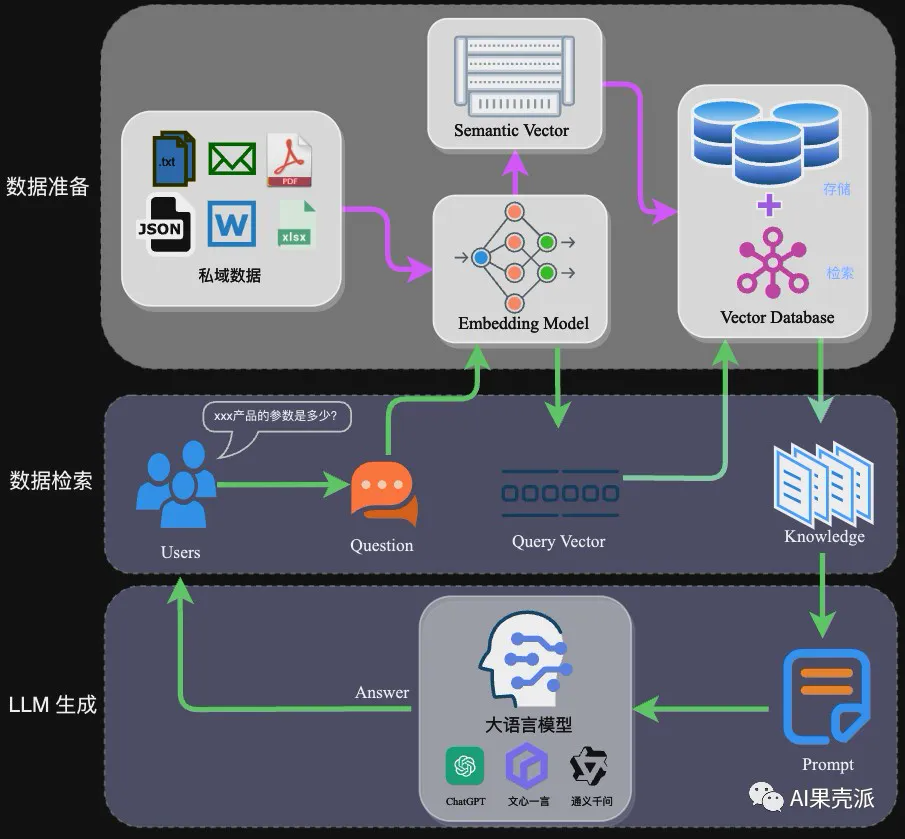
\includegraphics[height=.75\textheight]{pic/1.png}
        \caption{RAG, Retrieval Augmented Generation, 检索增强生成}
    \end{figure}
\end{frame}

\begin{frame}{发展}
    \begin{itemize}
        \item \sout{多租户}
        \item \sout{成本: 蒸馏, ...}
        \item \sout{向量数据库: ANN, 传统数据库, ...}
        \item LLM + (Priv) Data (e.g. 生物信息学)
        \item 向量化: Multimodal, 预处理, ...
    \end{itemize}
\end{frame}

\section{LLM}

\begin{frame}{GLEE}
    \begin{itemize}
        \item GLEE: General Object Foundation Model for Images and Videos at Scale
    \end{itemize}
\end{frame}

\begin{frame}{Visual Foundation Model}
    \begin{itemize}
        \item CLIP
        \item InternViT
        \item DINO
        \item ...
    \end{itemize}
\end{frame}

\begin{frame}{Multimodal: LLM + Visual Foundation Model}
    \begin{itemize}
        \item InternVL-Chat-V1.5: InternLM2	+ InternViT
        \item MiniCPM-Llama3-V2.5: Llama-3 + SigLip
        \item ...
    \end{itemize}
\end{frame}

\end{document}
